% !TeX program = xelatex
\documentclass{resume}
\ResumeName{谭邵杰}

\usepackage{graphicx}
\usepackage{tikz}
\linespread{1.04}\selectfont

\begin{document}

\ResumeContacts{
  \ResumeUrl{mailto:943648187@qq.com}{943648187@qq.com},%
  \ResumeUrl{https://shaojiemike.top}{shaojiemike.top},%
  \ResumeUrl{https://github.com/Kirrito-k423}{github.com/Kirrito-k423}%
}

\begin{tikzpicture}[remember picture,overlay]
  \node[anchor=north east,inner sep=1cm] at (current page.north east)
    {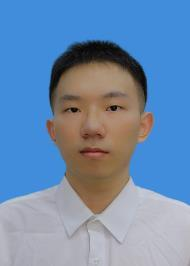
\includegraphics[width=1.85cm]{photo.jpg}};
\end{tikzpicture}

\ResumeTitle

\noindent 中国科学技术大学计算机科学与技术硕士，关注计算机体系结构、高性能计算、并行程序优化和 PIM 任务调度，具备从微架构分析、性能建模到多节点 CPU/GPU 优化的实践经验。

\section{教育经历}
\ResumeItem{中国科学技术大学}[计算机科学与技术（计算机体系结构）· 硕士][2021.09--2024.06]
\ResumeItem{中国科学技术大学}[计算机科学与技术 · 学士][2017.09--2021.06]

\section{研究与实习}
\ResumeItem{华为 2012 实验室}[暑期实习 · 存内计算 PIM 任务调度研究][2023.07]
\begin{itemize}
  \item 构建编译时性能模型，通过局部性聚类与连接性聚类减少数据移动。
  \item 结合并行度、访存端口压力等静态特征，在 PIM 与 CPU 间选择更优执行位置；仅依赖静态分析获得接近最优的调度结果。
\end{itemize}

\ResumeItem{中国科学技术大学 × 华为}[鲲鹏 920 基本块吞吐量建模][2021.09--2022.11]
\begin{itemize}
  \item 开发基本块吞吐量预测框架与基准测试集，整理吞吐量、延迟和端口压力等指令描述信息。
  \item 结合鲲鹏 920 微架构改进 llvm-mca 在 AArch64 下的精度，成果发表于 IEEE HPCC 2022。
\end{itemize}

\section{代表项目}
\ResumeItem{QuEST 多 GPU 量子门电路模拟}[ASC20-21 决赛一等奖][2020.11--2021.05]
\begin{itemize}
  \item 使用 CUDA-aware MPI 直接访问 GPU 显存，以多 stream 和 buffer 重叠计算与通信，并用 cuBLAS 替代向量点积和规约操作。
  \item 在 4 机 8 张 A100 上将规模从 30 拓展至 34 qubits，相较 CPU 系统节约 200+ GB 内存。
\end{itemize}

\ResumeItem{大数据串行应用的 CPU 多节点优化}[IPCC 2022 全国三等奖 · 5/130+][2022.07--2022.11]
\begin{itemize}
  \item 结合循环展开、手动向量化、OpenMP 与 MPI 实现多层并行，并优化数据布局、混合精度与 PSRS 等热点算法。
  \item 在 AMD EPYC 7452 平台实现双节点 10,000 倍、单节点最高 2,800,000 倍加速。
\end{itemize}

\section{技术能力}
\begin{itemize}
  \item \textbf{编程：}C、C++、Python、Shell；\textbf{并行计算：}MPI、OpenMP、CUDA、cuBLAS。
  \item \textbf{体系结构：}Intel/ARM 指令集、AArch64、CPU 微架构、PIM、性能建模；\textbf{分析：}汇编、向量化、缓存与带宽优化、llvm-mca。
\end{itemize}

\section{竞赛与论文}
\begin{itemize}
  \item ASC20-21 世界大学生超级计算机竞赛决赛一等奖；ISC21 国际大学生超级计算机竞赛决赛一等奖。
  \item Qingcai Jiang, \textbf{Shaojie Tan}, Zhenwei Cao, et al. ``Quantifying Throughput of Basic Blocks on ARM Microarchitectures by Static Code Analyzers: A Case Study on Kunpeng 920.'' \textbf{IEEE HPCC 2022}.
\end{itemize}

\end{document}

